\documentclass[11pt]{article}
\usepackage[T1]{fontenc}
\usepackage{lmodern}
\input{glyphtounicode}
\pdfgentounicode=1
\pdfglyphtounicode{parenleftbig}{0028}
\pdfglyphtounicode{parenrightbig}{0029}
\pdfglyphtounicode{bracketleftbig}{005B}
\pdfglyphtounicode{bracketrightbig}{005D}
\pdfglyphtounicode{vextendsingle}{23D0}
\pdfglyphtounicode{vextenddouble}{2016}
\pdfglyphtounicode{parenleftBig}{0028}
\pdfglyphtounicode{parenrightBig}{0029}
\pdfglyphtounicode{parenleftbigg}{0028}
\pdfglyphtounicode{parenrightbigg}{0029}
\pdfglyphtounicode{braceleftbigg}{007B}
\pdfglyphtounicode{bracerightbigg}{007D}
\pdfglyphtounicode{parenleftBigg}{0028}
\pdfglyphtounicode{parenrightBigg}{0029}
\pdfglyphtounicode{bracketleftBigg}{005B}
\pdfglyphtounicode{bracketrightBigg}{005D}
\pdfglyphtounicode{summationtext}{2211}
\pdfglyphtounicode{integraltext}{222B}
\pdfglyphtounicode{summationdisplay}{2211}
\pdfglyphtounicode{integraldisplay}{222B}
\pdfglyphtounicode{hatwide}{02C6}
\pdfglyphtounicode{tildewide}{02DC}
\pdfglyphtounicode{bracketleftBig}{005B}
\pdfglyphtounicode{bracketrightBig}{005D}
\pdfglyphtounicode{radicalbig}{221A}
\pdfglyphtounicode{radicalBig}{221A}
\pdfglyphtounicode{radicalBigg}{221A}
\pdfglyphtounicode{mapsto}{007C}
\pdfglyphtounicode{arrowhookleft}{21AA}
\pdfglyphtounicode{productdisplay}{220F}
\pdfglyphtounicode{circleplusdisplay}{2A01}
\pdfglyphtounicode{braceleftBig}{007B}
\pdfglyphtounicode{bracerightBig}{007D}
\pdfglyphtounicode{braceleftBigg}{007B}
\pdfglyphtounicode{bracerightBigg}{007D}
\pdfglyphtounicode{parenlefttp}{239B}
\pdfglyphtounicode{parenleftex}{239C}
\pdfglyphtounicode{parenleftbt}{239D}
\pdfglyphtounicode{parenrighttp}{239E}
\pdfglyphtounicode{parenrightex}{239F}
\pdfglyphtounicode{parenrightbt}{23A0}
\pdfglyphtounicode{bracketlefttp}{23A1}
\pdfglyphtounicode{bracketleftbt}{23A3}
\pdfglyphtounicode{bracketrighttp}{23A4}
\pdfglyphtounicode{bracketrightbt}{23A6}

\pdfglyphtounicode{uniontext}{22C3}
\pdfglyphtounicode{uniondisplay}{22C3}
\pdfglyphtounicode{intersectiontext}{22C2}
\pdfglyphtounicode{intersectiondisplay}{22C2}
\pdfglyphtounicode{braceleftbig}{007B}
\pdfglyphtounicode{bracerightbig}{007D}
\pdfglyphtounicode{bracelefttp}{23A7}
\pdfglyphtounicode{braceleftmid}{23A8}
\pdfglyphtounicode{braceleftbt}{23A9}
\pdfglyphtounicode{bracerighttp}{23AB}
\pdfglyphtounicode{bracerightmid}{23AC}
\pdfglyphtounicode{bracerightbt}{23AD}
\pdfglyphtounicode{braceex}{23AA}

\usepackage[margin=1in]{geometry}
\usepackage{amsmath,amssymb,amsthm,mathtools}
\usepackage{microtype}
\usepackage{enumitem}
\usepackage{booktabs,longtable,array}
\usepackage{xcolor}
\usepackage{tikz}
\usetikzlibrary{arrows.meta,positioning,fit}
\usepackage[numbers,sort&compress]{natbib}
\renewcommand{\bibfont}{\small}
\definecolor{linkblue}{RGB}{28,64,104}
\usepackage[colorlinks=true,linkcolor=linkblue,citecolor=linkblue,urlcolor=linkblue,breaklinks=true]{hyperref}
\usepackage{bookmark}
\providecommand{\doi}[1]{doi: \begingroup\urlstyle{rm}\href{https://doi.org/#1}{\nolinkurl{#1}}\endgroup}
\renewcommand{\bibsection}{\section*{\refname}\addcontentsline{toc}{section}{\refname}}
\hypersetup{pdftitle={Fixed Points of Nonexpansive Maps in Reflexive Banach Spaces},pdfsubject={The fixed point property for the given norm on a real reflexive Banach space},pdfauthor={OpenAI}}
\numberwithin{equation}{section}
\newtheorem{theorem}{Theorem}[section]
\newtheorem{lemma}[theorem]{Lemma}
\newtheorem{proposition}[theorem]{Proposition}
\newtheorem{corollary}[theorem]{Corollary}
\theoremstyle{definition}
\newtheorem{definition}[theorem]{Definition}
\theoremstyle{remark}
\newtheorem{remark}[theorem]{Remark}
\newcommand{\R}{\mathbb R}
\newcommand{\N}{\mathbb N}
\newcommand{\Z}{\mathbb Z}
\newcommand{\E}{\mathbb E}
\DeclarePairedDelimiter{\norm}{\lVert}{\rVert}
\DeclarePairedDelimiter{\abs}{\lvert}{\rvert}
\DeclareMathOperator{\Lip}{Lip}
\DeclareMathOperator{\conv}{conv}
\DeclareMathOperator{\diam}{diam}
\DeclareMathOperator{\dist}{dist}
\DeclareMathOperator{\supp}{supp}
\DeclareMathOperator{\sgn}{sgn}
\setlist{topsep=5pt,itemsep=3pt,parsep=0pt}
\setlength{\emergencystretch}{1.5em}
\allowdisplaybreaks[2]
\setcounter{tocdepth}{2}

\usepackage{accsupp}
\NewCommandCopy{\OriginalMapsto}{\mapsto}
\NewCommandCopy{\OriginalLongmapsto}{\longmapsto}
\NewCommandCopy{\OriginalHookrightarrow}{\hookrightarrow}
\renewcommand{\mapsto}{\BeginAccSupp{method=hex,unicode,ActualText=21A6}\OriginalMapsto\EndAccSupp{}}
\renewcommand{\longmapsto}{\BeginAccSupp{method=hex,unicode,ActualText=27FC}\OriginalLongmapsto\EndAccSupp{}}
\renewcommand{\hookrightarrow}{\BeginAccSupp{method=hex,unicode,ActualText=21AA}\OriginalHookrightarrow\EndAccSupp{}}

\title{Fixed Points of Nonexpansive Maps\\in Reflexive Banach Spaces}
\author{OpenAI}
\date{September 24, 2026}
\begin{document}
\maketitle
\begin{abstract}
Every nonexpansive selfmap of a nonempty closed bounded convex subset of a real reflexive Banach space has a fixed point. This resolves the reflexive-space fixed point problem for the given norm.
\end{abstract}
\section{Introduction}
\label{sec:introduction}

A Banach space has the \emph{fixed point property for nonexpansive maps}
if every nonexpansive selfmap of each nonempty closed bounded convex
subset has a fixed point. Here nonexpansiveness is measured in the given
norm. We prove the following theorem.

\begin{theorem}\label{thm:main}
Let $X$ be a real reflexive Banach space, and let $C\subseteq X$ be
nonempty, norm closed, bounded, and convex. If $F:C\to C$ satisfies
\[
  \norm{F(a)-F(b)}\le \norm{a-b}\qquad(a,b\in C),
\]
then $F$ has a fixed point.
\end{theorem}

Theorem~\ref{thm:main} establishes the positive assertion in the
reflexive-space fixed point problem for the given norm.

Bruck's theorem for commuting families gives a further consequence.

\begin{corollary}[Commuting families]\label{cor:commuting}
Let $X$ be a real reflexive Banach space, and let $C\subseteq X$ be
nonempty, norm closed, bounded, and convex. For any pairwise commuting
family $\mathcal S$ of nonexpansive selfmaps of $C$, the common fixed set
\[
  \operatorname{Fix}(\mathcal S)
  =\{x\in C:T(x)=x\text{ for every }T\in\mathcal S\}
\]
is nonempty and is a nonexpansive retract of $C$. That is, there is a
nonexpansive map $R:C\to\operatorname{Fix}(\mathcal S)$ that is the
identity on $\operatorname{Fix}(\mathcal S)$.
\end{corollary}

\begin{proof}
For the empty family, take $R=\operatorname{id}_C$. Otherwise,
Theorem~\ref{thm:main} applies to every nonempty closed bounded convex
subset $D$ of $C$, since a relatively norm-closed subset of the
norm-closed set $C$ is norm closed in $X$. Thus $C$
has Bruck's hereditary fixed point property and, by taking $D=C$, the
fixed point property. If $f:C\to C$ is nonexpansive and such a subset
$D$ is $f$-invariant, the same theorem applied to $f|_D$ gives a fixed
point in $D$. Hence $C$ also has Bruck's conditional fixed point
property. The ordinary fixed point and conditional fixed point properties
just proved, together with weak compactness of $C$ by reflexivity, satisfy
the corresponding hypotheses of \citet[Theorem~1]{Bruck1974}. That theorem
gives the claimed nonempty nonexpansive retract.
\end{proof}

The classical results of Browder and G\"ohde prove the fixed point
property for uniformly convex spaces
\cite{Browder1965,Gohde1965}. Kirk's theorem applies when the closed
bounded convex domain $C$ in a reflexive space has normal structure
\cite{Kirk1965}: every convex subset $D\subseteq C$ with more than one
point must contain a point $a$ with
$\sup_{z\in D}\norm{a-z}<\diam D$.
Kirk's proof uses the minimal invariant set reduction employed below,
with the normal-structure and center ideas of Brodski\u\i{} and
Milman credited there \cite[p.~1004]{Kirk1965}.
Karlovitz subsequently proved the fixed point property for a particular
norm on $\ell_2$ without normal structure \cite{Karlovitz1976}.
Thus these geometric conditions give sufficient criteria, but normal
structure is not necessary for the property.

Further results established the property for substantial classes beyond
the uniformly convex case. Maurey proved it for reflexive subspaces of
$L^1$ in the inherited norm \cite[Theorem~1]{Maurey1981}.
Lin proved the weak fixed point property for spaces with a
$1$-unconditional basis, meaning that changing signs of basis coefficients
preserves the norm \cite[Theorem~1]{Lin1985}. Here the weak fixed point
property restricts the domains to weakly compact convex sets; in a
reflexive space it is equivalent to the property considered here.
Garc\'ia-Falset, Llorens-Fuster, and Mazcu\~n\'an-Navarro proved the
property for uniformly nonsquare spaces \cite{GarciaFalset2006}; see also
the proof of \citet{Dowling2008}. This condition requires a
uniform gap below $1$ in at least one of
$\norm{(a+b)/2}$ and $\norm{(a-b)/2}$ for every pair $a,b$ in the unit ball.
These theorems concern the specified norm, with additional structure.

Two other results distinguish the hypotheses of
Theorem~\ref{thm:main}. Alspach constructed a weakly compact convex
subset of $L_1[0,1]$ with a fixed-point-free nonexpansive selfmap
\cite{Alspach1981}. Weak compactness of the domain in an arbitrary
Banach space is therefore insufficient. Dom\'inguez Benavides proved
that every reflexive Banach space admits an equivalent norm with the
fixed point property \cite[Corollary~1]{Benavides2009}. A change of norm
can change which maps are nonexpansive; the theorem here concerns the
original norm.

Hanebaly previously proposed a proof of this same original-norm
assertion \cite[Theorem~1]{Hanebaly2019}, and subsequently announced
a further proof \cite{Hanebaly2021}. More recent discussion of the
general question appears in \citet[Section~1]{Nourouzi2026}, who
records it as unresolved. These statements of the literature are distinct
from the argument given here. Our proof proceeds through an adaptive
anchor, compact families of predicted outputs, and weighted switching
on a tree.

\paragraph{The argument.}
Suppose a counterexample exists. The classical minimal invariant set
method reduces the problem to a separable weakly compact convex set
$K$ of diameter one. Approximate fixed points in $K$ become asymptotically
diametral: their distance from every prescribed point of $K$ tends to one.
This is the Goebel--Karlovitz lemma
\cite{Goebel1975,Karlovitz1976}, proved in
Lemma~\ref{lem:diametral} below.

The proof uses this diametral behavior through two constructions.
First, a compact semigroup of nonexpansive maps provides an anchor
$x\in K$. Finite convex combinations of increasingly accurate
approximate fixed point images of $x$ can return arbitrarily close
to $x$, even when the accuracy required at each choice depends on
all previous choices. Second, these images label an ordered tree.
At each node, a compact family contains the required weak limits of
ideal root outputs, with parameters for the convex coefficients still
to be chosen. These outputs model the state after a prescribed block
of leaves has been replaced by a common approximate fixed point.

Replacing the leaves from right to left gives a sequence of actual
root outputs. Their consecutive differences telescope, although
the maps defining the tree are nonlinear. Weighted estimates for
these differences produce, at every finite depth, one vector
detected by all the functionals along a branch. A summable error
budget controls the total weighted deficit without a lower bound
on the individual branch weights. Finally, weak compactness of the
unit ball of $\overline{\operatorname{span}}(K-K)$ gives one vector
detected along an infinite branch, while the same functionals tend
pointwise to zero on that space.

The adaptive choice of the anchor images, the compact families of
predicted outputs, and the weighted telescoping estimate are the
parts of the argument that go beyond the classical diametral
reduction. They are formulated separately so that their dependence
on convexity, nonexpansiveness, and compactness is explicit.
Section~\ref{sec:prelim} supplies the compactness and separation
facts used throughout, with their proofs in
Appendix~\ref{app:foundations}; Sections~\ref{sec:anchor} and~\ref{sec:tree}
construct the anchor and tree; Section~\ref{sec:switching} proves
the switching estimate and completes the contradiction.

\section{Weak compactness and a minimal invariant set}\label{sec:prelim}

We first record the functional-analytic facts needed below, including their
compactness ingredients. The weak topology of a normed space is the topology
generated by its continuous linear functionals. Its continuous dual $X^*$
carries the operator norm, and $X^{**}=(X^*)^*$. Reflexivity means that
the canonical map $J_X:X\to X^{**}$, defined by $(J_Xx)(f)=f(x)$, is onto.
We write
$\overline{\conv} A$ for the norm-closed convex hull of $A$.

\begin{lemma}\label{lem:weak-facts}
Let $X$ be a real normed space.
\begin{enumerate}
\item Every $v\in X$ has a norming functional: there is $f\in X^*$ with
      $\norm{f}\leq 1$ and $f(v)=\norm{v}$. Every norm-closed convex set is
      weakly closed, and the norm is weakly lower semicontinuous.
\item On a finite Cartesian power of $X$, the weak topology is the product
      weak topology. The norm and weak closures of a convex set coincide.
\item If $X$ is reflexive and complete, every norm-closed bounded convex
      subset of $X$ is weakly compact. Arbitrary products of compact
      Hausdorff spaces are compact.
\end{enumerate}
\end{lemma}

The proof, including the compactness details, is given in
Appendix~\ref{app:foundations}.


Throughout, $\N=\{1,2,\ldots\}$. We use the following limit convention.
A proper filter is a family of
subsets closed under finite intersections and supersets, containing the
whole set but not the empty set. An \emph{ultrafilter} is maximal under
inclusion among proper filters. Fix an ultrafilter $\mathcal U$ on $\N$
extending the filter of cofinite sets. It contains no finite set and is
therefore \emph{free}. For a sequence $(a_j)$, the notation
$a=\lim_{j\to\mathcal U}a_j$ means that
$\{j:a_j\in V\}\in\mathcal U$ for every neighborhood $V$ of $a$.
The existence of such $\mathcal U$, and existence and uniqueness of
these limits in compact Hausdorff spaces, are proved in
Appendix~\ref{app:foundations}.

\begin{samepage}
\begin{lemma}\label{lem:reduction}
If Theorem~\ref{thm:main} fails, there are a nonempty separable,
weakly compact convex set $K$ and a nonexpansive map $T:K\to K$ without
a fixed point such that $K$ has no proper nonempty norm-closed convex
$T$-invariant subset. We may take $\diam K=1$ by scalar normalization.
Moreover, the weak topology on $K$ is metrizable. For
\[
          Y=\overline{\operatorname{span}}(K-K),
          \qquad B_Y=\{y\in Y:\norm{y}\leq1\},
\]
the ball $B_Y$ is weakly compact, and $Y$ is separable.
\end{lemma}
\end{samepage}

\begin{proof}
Start with a fixed-point-free map $F:C\to C$ as in the theorem and a point
$a\in C$. Set $C_0=\{a\}$ and
$C_{n+1}=\overline{\conv}(C_n\cup F(C_n))$.
These sets are increasing and separable: continuous images of separable
sets are separable, and rational convex combinations of a countable dense
set are dense in its convex hull. Hence
$C'=\overline{\bigcup_n C_n}$ is separable, bounded, closed, and convex.
Norm continuity of $F$ gives $F(C')\subseteq C'$, and
Lemma~\ref{lem:weak-facts} makes $C'$ weakly compact.

Every decreasing chain of nonempty norm-closed convex invariant subsets
of $C'$ has a nonempty intersection, by weak compactness and the finite
intersection property. The intersection is again closed, convex, and
invariant. Zorn's Lemma, with inclusion reversed, therefore supplies a
minimal such set $K$. Put $T=F|_K$. Its diameter $d$ is positive, since
a singleton invariant set would give a fixed point. From now on express
distances in units of $d$, writing $\norm{\cdot}$ for the original norm
divided by $d$. This scalar normalization preserves the topologies,
nonexpansiveness, and fixed points; it makes $\diam K=1$.

Choose a norm-dense sequence $(z_i)_{i\geq1}$ in $K$. Its pairwise
differences have dense linear span in $Y$, so $Y$ is separable.
Choose a dense sequence $(u_j)$ in the unit sphere of $Y$ and norming
functionals $g_j\in X^*$ for these vectors. They separate points of $Y$:
if $\norm{v}=1$ and $\norm{v-u_j}<1/2$, then $g_j(v)>1/2$.
Thus the map $a\mapsto(g_j(a))_{j\geq1}$ continuously injects weakly
compact $K$ into $\R^{\N}$. The latter is metrizable, for example by
$\sum_j2^{-j}\min\{1,\abs{s_j-t_j}\}$.
The injection is a homeomorphism onto its image, since compact subsets
of a Hausdorff space are closed. Hence the weak topology on $K$ is
metrizable. Finally $B_Y$ is a norm-closed bounded convex subset of $X$,
so is weakly compact by Lemma~\ref{lem:weak-facts}. Its inherited weak
topology equals its intrinsic weak topology: restriction gives one
inclusion of continuous functionals, and the extension argument in
Lemma~\ref{lem:weak-facts} gives the other.
\end{proof}

We argue by contradiction for the remainder of the proof and fix
$K,T,Y$, and $(z_i)$ as in Lemma~\ref{lem:reduction}.
A sequence $(u_j)$ in $K$ is an \emph{approximate fixed point sequence}
if $\norm{Tu_j-u_j}\to0$.
The next lemma is the diameter lemma of Goebel and Karlovitz
\cite{Goebel1975,Karlovitz1976}; we include its proof.
Karlovitz also records independent development of this lemma by
P.~M.~Fitzpatrick \cite[p.~159]{Karlovitz1976}.

\begin{lemma}\label{lem:diametral}
Every approximate fixed point sequence $(u_j)$ satisfies
\[
                     \lim_{j\to\infty}\norm{u_j-z}=1
                     \qquad(z\in K).
\]
\end{lemma}

\begin{proof}
First $K=\overline{\conv}T(K)$: this hull is nonempty and contained in
$K$, and its image under $T$ is contained in $T(K)$ and hence in the hull.
Minimality applies. Consider on $K$ the functions
\[
       s(z)=\sup_{w\in K}\norm{z-w},
       \qquad r(z)=\limsup_j\norm{z-u_j}.
\]
Both are convex and $1$-Lipschitz. For a fixed center, the distance
function is convex and continuous, so its supremum is unchanged on
passing to a norm-closed convex hull. The hull identity and
nonexpansiveness give
\[
 s(Tz)=\sup_{w\in K}\norm{Tz-Tw}\leq s(z),
 \qquad r(Tz)\leq r(z),
\]
where the second inequality also uses $\norm{Tu_j-u_j}\to0$.
Every nonempty sublevel set of either function is norm closed, convex,
and invariant. If the function had two different values, a sublevel
strictly between them would contradict minimality. Both functions
are therefore constant, and $s=1$ because its supremum is $\diam K$.
Write $r=R\leq1$.

Take the weak $\mathcal U$-limit $a\in K$ of $(u_j)$. For every $z\in K$
and $\eta>0$, all sufficiently large $j$ satisfy
$\norm{z-u_j}\leq R+\eta$. The corresponding closed ball is weakly
closed and the cofinite sets belong to $\mathcal U$, so
$\norm{z-a}\leq R+\eta$. Letting $\eta$ decrease to zero and taking
the supremum over $z$ gives $1=s(a)\leq R$, hence $R=1$.
This argument applies to every subsequence of $(u_j)$, since each is
again an approximate fixed point sequence. As all distances are at most
$1$, a failure of the asserted limit would give a subsequence bounded
above by $1-\eta$ for some $\eta>0$, contradicting its limsup of $1$.
\end{proof}

\begin{lemma}\label{lem:compact-detector}
For every nonempty norm-compact set $E\subseteq K$ and every
$\varepsilon>0$, there exists $\delta>0$ such that each $y\in K$ with
$\norm{Ty-y}\leq\delta$ admits a single $f\in X^*$, $\norm{f}\leq1$,
satisfying
\[
                     f(y-z)\geq1-\varepsilon\qquad(z\in E).
\]
\end{lemma}

\begin{proof}
Choose an $\varepsilon/2$-net $a_1,\ldots,a_m$ in $E$ and set
$a=m^{-1}\sum_{i=1}^m a_i\in K$. Lemma~\ref{lem:diametral} implies
that, for some $\delta>0$,
\[
 \norm{Ty-y}\leq\delta
       \quad\Longrightarrow\quad
 \norm{y-a}\geq1-\frac{\varepsilon}{2m}.
\]
Indeed, otherwise choosing a violating point with defect at most $1/j$
for each $j$ would contradict that lemma. Choose a norming functional
$f$ for $y-a$. The numbers $f(y-a_i)$ are all at most $1$, whereas
their sum is $m f(y-a)\geq m-\varepsilon/2$. Each is therefore at least
$1-\varepsilon/2$. For $z\in E$, take $a_i$ with
$\norm{z-a_i}<\varepsilon/2$ and use $\norm{f}\leq1$ to obtain the
claimed bound.
\end{proof}

\section{An anchor for successive choices}
\label{sec:anchor}

We construct a point $x\in K$ and a family of nonexpansive maps whose
images of $x$ have two useful properties.  Their fixed point defects can
be made arbitrarily small, even after additional requirements have been
imposed by earlier choices, and finite convex combinations of these
images can return arbitrarily close to $x$ in norm.  The construction
uses compactness in a space of maps; finite simultaneous approximation
in norm will justify the compositions that occur there.

\subsection{Resolvents and displacement estimates}

We begin with the classical resolvent construction; see
\citet[pp.~75--76]{Goebel1975}.

\begin{lemma}[Resolvents]
\label{lem:resolvents}
For every $n\geq 1$ and $a\in K$, there is a unique point $R_n(a)\in K$
satisfying
\begin{equation}
\label{eq:resolvent-definition}
 R_n(a)=\frac{a}{n}+\left(1-\frac1n\right)T R_n(a).
\end{equation}
The map $R_n:K\to K$ is nonexpansive, and
\begin{equation}
\label{eq:resolvent-estimates}
 \norm{T R_n(a)-R_n(a)}\leq\frac1n,
 \qquad
 \norm{R_n(a)-a}\leq(n-1)\norm{Ta-a}
 \quad(a\in K).
\end{equation}
\end{lemma}

\begin{proof}
For $n=1$, the defining equation gives $R_1(a)=a$.  For $n>1$, the map
\[
 u\longmapsto \frac{a}{n}+\left(1-\frac1n\right)Tu
\]
takes the complete set $K$ into itself and has Lipschitz constant
$q=1-1/n<1$.  Starting from any point of $K$, its iterates have successive
displacements bounded by $q^r$ times the first displacement.  The
geometric series shows that the iterates are Cauchy.  Their limit solves
\eqref{eq:resolvent-definition} by norm continuity.  Two solutions have
distance at most $q$ times their distance and therefore coincide.

For $u=R_n(a)$ and $v=R_n(b)$, comparison of their equations gives
\[
 \norm{u-v}\leq\frac1n\norm{a-b}
              +\left(1-\frac1n\right)\norm{u-v},
\]
which proves nonexpansiveness.  The identity
$Tu-u=(Tu-a)/n$ and $\diam K=1$ give the first estimate in
\eqref{eq:resolvent-estimates}.  For the second, the defining equation
and nonexpansiveness of $T$ give
\[
 \norm{u-a}
 \leq\left(1-\frac1n\right)
       \bigl(\norm{u-a}+\norm{Ta-a}\bigr).
\]
Rearranging proves the claim.
\end{proof}

Let $\mathcal G$ be the family generated by the identity map and the
maps $R_n$ using finitely many compositions and pointwise finite convex
combinations.  Every member of $\mathcal G$ is a nonexpansive selfmap of
$K$.  Moreover, for each $G\in\mathcal G$ there is a finite constant
$c_G\geq0$ such that
\begin{equation}
\label{eq:map-displacement}
 \norm{G(a)-a}\leq c_G\norm{Ta-a}
 \qquad(a\in K).
\end{equation}
For the generators, take $c_{\mathrm{Id}}=0$ and $c_{R_n}=n-1$.
Convex combinations preserve the estimate with the same convex
combination of the constants.  For compositions, nonexpansiveness gives
\begin{align*}
 \norm{G_1(G_2(a))-a}
 &\leq\norm{G_1(G_2(a))-G_1(a)}+\norm{G_1(a)-a}\\
 &\leq\norm{G_2(a)-a}+\norm{G_1(a)-a}\\
 &\leq(c_{G_2}+c_{G_1})\norm{Ta-a}.
\end{align*}
This proves \eqref{eq:map-displacement} throughout $\mathcal G$.
The same composition estimate underlies Bruck's semigroup of maps
asymptotically fixing a common approximate fixed point sequence
\cite[p.~115]{Bruck1975}.

For $m\geq1$, define the tail family
\begin{equation}
\label{eq:tail-family}
 \mathcal H_m
   =\{R_n\circ G:n\geq m,\ G\in\mathcal G\}.
\end{equation}
These families are nonempty, contained in $\mathcal G$, and decreasing
with $m$.  Their outer resolvents give the uniform bound
\begin{equation}
\label{eq:tail-defect}
 \norm{T h(a)-h(a)}\leq\frac1m
 \qquad(h\in\mathcal H_m,\ a\in K).
\end{equation}

\subsection{A compact semigroup of maps}


Convex semigroups of nonexpansive maps, with the topology of pointwise
weak convergence, were studied by Bruck \cite{Bruck1975}. His
common-fixed-point theorem assumes strict convexity and pairwise
intersection of the closed convex hulls of the ranges of the maps.
Here the semigroup will supply an idempotent anchor, through Ellis's
lemma; the tree and switching arguments will then produce the fixed
point. The composition estimates below keep the needed continuity
properties explicit.

Give $K^K$, the set of all maps from $K$ into itself, the topology of
pointwise weak convergence.  It is a compact Hausdorff space by the
product compactness in Lemma~\ref{lem:weak-facts}.  We write
$\overline{\mathcal B}^{\,\mathrm{pw}}$ for closure in this space.

\begin{lemma}[Finite simultaneous approximation]
\label{lem:finite-tuples}
Let $\mathcal B\subseteq K^K$ be a nonempty convex family of
nonexpansive maps.  Every map
$h\in\overline{\mathcal B}^{\,\mathrm{pw}}$ is nonexpansive.
For any integer $q\geq1$, points $a_1,\ldots,a_q\in K$, and
$\delta>0$, there is a single
$g\in\mathcal B$ such that
\[
 \max_{1\leq i\leq q}\norm{g(a_i)-h(a_i)}<\delta.
\]
\end{lemma}

\begin{proof}
For each fixed pair $a,b\in K$, the condition
$\norm{h(a)-h(b)}\leq\norm{a-b}$ is closed in the pointwise weak
topology: evaluation at $a,b$ and subtraction are weakly continuous,
and norm balls are weakly closed.  Intersecting these conditions over
all pairs proves the first assertion.

For the second, consider the convex subset
\[
 V=\{(g(a_1),\ldots,g(a_q)):g\in\mathcal B\}\subseteq X^q.
\]
The tuple $(h(a_1),\ldots,h(a_q))$ belongs to its weak closure, by
continuity of evaluation.  The weak topology of the finite Banach
product $X^q$ is the product of its coordinate weak topologies: each
continuous linear functional on $X^q$ is the sum of its coordinate
restrictions.  By separation, the weak and norm closures of a convex
subset of $X^q$ agree.  Applying this fact with the maximum coordinate
norm gives one element of $V$ satisfying all the desired inequalities.
\end{proof}

We will also use the following elementary compact semigroup argument,
the right-translation version of \citet[Lemma~1, p.~402]{Ellis1958}.
Ellis uses the opposite convention for composition.
Here a semigroup is a set with an associative multiplication.

\begin{lemma}[Idempotent in a compact semigroup]
\label{lem:idempotent}
Let $S$ be a nonempty compact Hausdorff semigroup.  Suppose that, for
each $p\in S$, the right translation $h\mapsto hp$ is continuous.
Then $S$ contains an idempotent: an element $p$ with $p^2=p$.
\end{lemma}

\begin{proof}
The intersection of a chain of nonempty compact subsemigroups of $S$
is nonempty by compactness and is again a compact subsemigroup.
Zorn's lemma therefore gives a minimal nonempty compact subsemigroup
$S'\subseteq S$.  Fix $p\in S'$.  The set $S'p$ is a nonempty compact
subset of $S'$ by continuity of right translation.  It is a
subsemigroup because
\[
 (ap)(bp)=(apb)p\in S'p\qquad(a,b\in S').
\]
Minimality gives $S'p=S'$, so in particular there is an $h\in S'$ with
$hp=p$.  The set
\[
 E=\{h\in S':hp=p\}
\]
is thus nonempty.  It is compact by continuity of right translation
and is a subsemigroup, since $hp=kp=p$ implies
$(hk)p=h(kp)=hp=p$.  Minimality gives $E=S'$, and $p\in E$ proves
$p^2=p$.
\end{proof}

Set
\begin{equation}
\label{eq:map-closures}
 A_m=\overline{\conv\mathcal H_m}^{\,\mathrm{pw}},
 \qquad A=\bigcap_{m\geq1}A_m.
\end{equation}

\begin{proposition}[An anchor point]
\label{prop:anchor}
The set $A$ is a nonempty compact semigroup of nonexpansive selfmaps
of $K$ and contains an idempotent $P$.  There is a point $x\in K$ with
$P(x)=x$ such that the nonempty weakly compact set
\begin{equation}
\label{eq:anchor-tail-set}
 D_x=\bigcap_{m\geq1}
       \overline{\{h(x):h\in\mathcal H_m\}}^{\,\mathrm{weak}}
\end{equation}
satisfies
\begin{equation}
\label{eq:anchor-convex-hull}
 x\in\overline{\conv D_x}^{\,\norm{\cdot}}.
\end{equation}
\end{proposition}

\begin{proof}
The sets $A_m$ are nonempty, compact, and decreasing.  Every member
is nonexpansive by Lemma~\ref{lem:finite-tuples}.

First, $\conv\mathcal H_m$ is closed under composition.  Indeed, if
\[
 g=\sum_{r=1}^s\lambda_r(R_{n_r}\circ G_r)
 \in\conv\mathcal H_m,
 \qquad k\in\conv\mathcal H_m,
\]
then $k\in\mathcal G$ and
\[
 g\circ k
 =\sum_{r=1}^s\lambda_r\bigl(R_{n_r}\circ(G_r\circ k)\bigr)
 \in\conv\mathcal H_m.
\]
This identity distributes precomposition over the outer convex
combination.

To pass to $A_m$, fix $h,k\in A_m$, arguments $a_1,\ldots,a_q\in K$,
and $\delta>0$.  Lemma~\ref{lem:finite-tuples} gives
$k_\delta,h_\delta\in\conv\mathcal H_m$ with
\[
 \max_i\norm{k_\delta(a_i)-k(a_i)}<\delta,
 \qquad
 \max_i\norm{h_\delta(k(a_i))-h(k(a_i))}<\delta.
\]
The second application uses the fixed arguments $k(a_i)$.
Nonexpansiveness of $h_\delta$ then gives
\begin{align*}
 &\norm{h_\delta(k_\delta(a_i))-h(k(a_i))}\\
 &\quad\leq
   \norm{h_\delta(k_\delta(a_i))-h_\delta(k(a_i))}
   +\norm{h_\delta(k(a_i))-h(k(a_i))}\\
 &\quad\leq\norm{k_\delta(a_i)-k(a_i)}
   +\norm{h_\delta(k(a_i))-h(k(a_i))}
   <2\delta.
\end{align*}
The composition $h_\delta\circ k_\delta$ belongs to
$\conv\mathcal H_m$.  Since the finite arguments and $\delta$ were
arbitrary, these simultaneous norm approximations imply
$h\circ k\in A_m$.

Thus $A$ is a nonempty compact semigroup, by the nested intersection
property.  For fixed $k\in A$, the right translation
$h\mapsto h\circ k$ is continuous in the pointwise weak topology:
its value at an argument $a$ is the evaluation of $h$ at the fixed
argument $k(a)$.  Lemma~\ref{lem:idempotent} supplies $P\in A$ with
$P\circ P=P$.  Choose any $a\in K$ and set $x=P(a)$; then $P(x)=x$.

Write
\[
 B_m=\overline{\{h(x):h\in\mathcal H_m\}}^{\,\mathrm{weak}}.
\]
These are nonempty nested weakly compact subsets of $K$, so
$D_x=\bigcap_m B_m$ is nonempty and weakly compact.  Since
$P\in A_m$, Lemma~\ref{lem:finite-tuples} at the single argument $x$
shows that
\[
 x=P(x)\in
 \overline{\conv\{h(x):h\in\mathcal H_m\}}^{\,\norm{\cdot}}
 \subseteq\overline{\conv B_m}^{\,\norm{\cdot}}.
\]
Consequently, for each $\ell\in X^*$,
\[
 \max_{z\in B_m}\ell(z)\geq\ell(x).
\]
The maximum exists because $B_m$ is weakly compact.  The sets
$B_m\cap\{z:\ell(z)\geq\ell(x)\}$ are nonempty nested compact sets;
their intersection gives a point of $D_x$ at which
$\ell\geq\ell(x)$.  Hence
\[
 \sup_{z\in D_x}\ell(z)\geq\ell(x)\qquad(\ell\in X^*).
\]
If \eqref{eq:anchor-convex-hull} failed, separation from the
norm-closed convex hull of $D_x$ would give a functional violating
this inequality.  This proves the proposition.
\end{proof}

\subsection{Successive choices with prescribed thresholds}

Fix the point $x$ supplied by Proposition~\ref{prop:anchor}.  Its
convex-hull property permits each new map to be selected at a scale
that depends on all preceding choices.

\begin{lemma}[Adaptive finite selection]
\label{lem:adaptive-selection}
Let $\tau>0$.  There is a successive selection procedure with the
following property.  Before the $i$th map is chosen, prescribe any
finite integer $m_i\geq1$, allowing this prescription to depend on the
entire previous history and on any auxiliary data already fixed at
that stage.  The procedure chooses $G_i\in\mathcal H_{m_i}$ and
terminates after finitely many steps, say $M$, with nonnegative
coefficients $\beta_1,\ldots,\beta_M$ such that
\begin{equation}
\label{eq:adaptive-return}
 \sum_{i=1}^M\beta_i=1,
 \qquad
 \norm*{\sum_{i=1}^M\beta_iG_i(x)-x}<\tau.
\end{equation}
The coefficients are assigned on termination.  Removing zero
coefficients gives a nonempty list with positive coefficients,
in the original order of selection.
\end{lemma}

\begin{proof}
Choose $d_1,\ldots,d_q\in D_x$ and nonnegative coefficients
$\lambda_1,\ldots,\lambda_q$ summing to $1$ such that
\[
 \norm*{\sum_{r=1}^q\lambda_rd_r-x}<\frac\tau2.
\]
Fix a metric $\rho$ inducing the weak topology on $K$.  Cycle through
the targets $d_1,\ldots,d_q$: at step $i$, let $r(i)$ be the member of
$\{1,\ldots,q\}$ congruent to $i$ modulo $q$.  Once the threshold
$m_i$ has been prescribed, the membership
\[
 d_{r(i)}\in
 \overline{\{h(x):h\in\mathcal H_{m_i}\}}^{\,\mathrm{weak}}
\]
allows a choice $G_i\in\mathcal H_{m_i}$ with
\[
 \rho\bigl(G_i(x),d_{r(i)}\bigr)<\frac1i.
\]
Any auxiliary choices associated with this map may now be made before
the next threshold is prescribed.  Stop as soon as the convex hull
of the selected images comes within distance $\tau$ of $x$.

Suppose that the procedure never stops, and let
\[
 C_0=\overline{\conv\{G_i(x):i\geq1\}}^{\,\norm{\cdot}}.
\]
For each $r$, the subsequence assigned to target $d_r$ converges
weakly to $d_r$.  The set $C_0$ is weakly closed by separation, so
it contains every $d_r$ and their convex combination
$\sum_r\lambda_rd_r$.  By the definition of $C_0$, a finite convex
combination of the selected images is within $\tau/2$ of this last
point.  It is therefore within $\tau$ of $x$.  All its indices occur
in some finite prefix of the selection, contradicting the stopping
rule.  The procedure thus terminates, and a convex combination at
the stopping step supplies \eqref{eq:adaptive-return}.  Deleting its
zero coefficients leaves the stated positive list.
\end{proof}

By \eqref{eq:tail-defect}, the threshold at each selection may impose
any positive upper bound on the defect of that individual image.
The convex coefficients in Lemma~\ref{lem:adaptive-selection} provide
the return to $x$ in norm.

Finally, fix once and for all the sequence
\begin{equation}
\label{eq:terminal-sequence}
 b_j=R_j(x)\qquad(j\geq1).
\end{equation}
Lemma~\ref{lem:resolvents} and \eqref{eq:map-displacement} give
\begin{equation}
\label{eq:terminal-displacement}
 \norm{Tb_j-b_j}\leq\frac1j,
 \qquad
 \norm{G(b_j)-b_j}\leq\frac{c_G}{j}
 \quad(G\in\mathcal G).
\end{equation}
Thus every fixed finite family of maps in $\mathcal G$ acts
arbitrarily close to the identity at a common sufficiently late
$b_j$.  This sequence will be used throughout the remaining
construction.

\section{A tree of maps and separating functionals}
\label{sec:tree}

Fix the point $x$ supplied by Proposition~\ref{prop:anchor} and the
sequence $b_j=R_j(x)$ from Section~\ref{sec:anchor}.  We construct a
single infinite tree.  Each node carries a map in $\mathcal G$, and
each nonroot node also carries a functional.  The maps will allow a
subtree to approximate its prescribed label or to transmit a common
point $b_j$.  Each functional must be chosen before the weights in its own
sibling group are assigned.  A family of possible root outputs parameterized
by a compact finite-dimensional set makes this order of choices possible.

\subsection{Evaluation on an ordered tree}

The root is denoted by $r$, and $L_k$ denotes the finite, nonempty
level of depth $k$, with $L_0=\{r\}$.  Every node has a finite,
nonempty ordered list of children.  The order on $L_{k+1}$ is obtained
by placing these lists consecutively in the order of their parents
in $L_k$.  Write $\widehat v$ for the parent of $v$, and $p\prec v$
when $p$ is a proper ancestor of $v$.  In particular, $\prec$ does
not denote the order within a level.

Each node $v$ is assigned a map $G_v\in\mathcal G$ and the point
$y_v=G_v(x)$.  At the root, $G_r=\operatorname{Id}_K$ and $y_r=x$.
Each nonroot node has a weight $\alpha_v>0$, with
\[
  \sum_{\widehat v=u}\alpha_v=1
  \qquad\text{for every node }u.
\]
Given outputs at the children of $u$, the output at $u$ is
\begin{equation}
  H_u=G_u\left(\sum_{\widehat v=u}\alpha_v H_v\right).
  \label{eq:tree-rule}
\end{equation}
Every output belongs to $K$.  If outputs $(H_v)_{v\in L_k}$ are
prescribed at a cutoff level, let $\Phi_k((H_v)_{v\in L_k})$ be the
root output obtained by applying this rule strictly above that level.
Thus $\Phi_0(H_r)=H_r$; a map at the cutoff itself is not applied
again.

Define the path weights by
\[
  W_r=1,\qquad W_v=W_{\widehat v}\alpha_v\quad(v\ne r).
\]
An induction gives $\sum_{v\in L_k}W_v=1$.  More generally, the
sum of the weights at any later level below a given node is the
weight of that node.  Nonexpansiveness and the triangle inequality
also give, by induction up the tree,
\begin{equation}
 \norm{\Phi_k((H_v)) - \Phi_k((H'_v))}
 \le \sum_{v\in L_k}W_v\norm{H_v-H'_v}.
 \label{eq:tree-sensitivity}
\end{equation}
Indeed, at each parent the difference is at most the weighted sum of
the child differences.  Iterating multiplies the weights along each
path.  Consequently the root error is at most the largest cutoff
error, and changing only the output at $v\in L_k$ changes the root
by at most $W_v$ times the change at $v$.

\subsection{Predictions using earlier candidates}

We first describe the information associated with a candidate node
$v$ of depth $k\ge1$ during construction.  At this stage, all levels
of depth less than $k$, including their maps and weights, have
already been fixed.  Candidates at depth $k$ are selected one parent
group at a time, from left to right, and within each group in their
order of selection.  Let $I_v$ be the finite list of earlier
depth-$k$ candidates.  We retain their points $y_h$ and parent labels
even if some of these candidates have already been discarded from
the tree.  The map $G_v$ and point $y_v$ have not yet been chosen.

The later switching experiment replaces leaf outputs from right to
left. If $v$ is retained, then just after its block has switched, the \emph{ideal}
cutoff state uses $y_h$ at nodes strictly left of $v$ and a common
point $b$ at $v$ and to its right. The actual subtree outputs will
approximate these prescribed values. We must describe the root
outputs of this ideal state before the current level's weights and
later children are known.

Put
\[
 \Theta_v=\left\{(\theta_h)_{h\in I_v}:
    \theta_h\ge0,\quad
    \sum_{\substack{h\in I_v\\\widehat h=p}}\theta_h\le1
       \quad(p\in L_{k-1})\right\}.
\]
This is a compact subset of a finite-dimensional space.  If $I_v$
is empty, it consists of the single empty tuple.  For $b\in K$ and
$\theta\in\Theta_v$, set
\begin{equation}
 \begin{split}
 a_{v,p}(b;\theta)
   &=b+\sum_{\substack{h\in I_v\\\widehat h=p}}
                     \theta_h(y_h-b),\qquad p\in L_{k-1},\\
 Q_v(b;\theta)
   &=\Phi_{k-1}\bigl((G_p(a_{v,p}(b;\theta)))_{p\in L_{k-1}}\bigr).
 \end{split}
 \label{eq:prediction-definition}
\end{equation}
Each $a_{v,p}$ is a convex combination of $b$ and the earlier
candidates belonging to $p$, so it lies in $K$.  The residual
coefficient of $b$ represents all children whose outputs are to be
replaced by that common point.  Only maps and weights at depths less
than $k$ enter the evaluation of $Q_v$.

For fixed $v$, the map $\theta\mapsto Q_v(b;\theta)$ is norm
Lipschitz, uniformly over $b\in K$.  In fact, since $\diam K=1$,
\[
 \norm{a_{v,p}(b;\theta)-a_{v,p}(b;\eta)}
 \le \sum_{\substack{h\in I_v\\\widehat h=p}}
                      \abs{\theta_h-\eta_h}.
\]
Applying the nonexpansive maps $G_p$ and
Equation~\eqref{eq:tree-sensitivity} gives
\begin{equation}
 \norm{Q_v(b;\theta)-Q_v(b;\eta)}
 \le \sum_{h\in I_v}\abs{\theta_h-\eta_h}.
 \label{eq:prediction-lipschitz}
\end{equation}
For each $\theta$, weak compactness of $K$ gives the limit
\[
 Z_v(\theta)=\operatorname*{w-lim}_{j\to\mathcal U}
                      Q_v(b_j;\theta)\in K.
\]
The difference of the two sequences at $\theta$ and $\eta$
converges weakly along $\mathcal U$ to
$Z_v(\theta)-Z_v(\eta)$.  The norm ball of radius
$\sum_{h\in I_v}\abs{\theta_h-\eta_h}$ is weakly closed, so
Equation~\eqref{eq:prediction-lipschitz} implies the same bound for
$\norm{Z_v(\theta)-Z_v(\eta)}$.  Thus $Z_v$ is continuous into the
norm topology, and
\begin{equation}
 E_v=\{z_1,\ldots,z_k\}\cup Z_v(\Theta_v)
 \label{eq:tree-detector-set}
\end{equation}
is a nonempty norm-compact subset of $K$.  It is completely
determined before $G_v$ is selected. The dense test points will force
the branch functionals to tend to zero on the differences $z_i-z_j$,
and hence on $Y$; the compact prediction image provides comparison
limits for block detection. This argument takes weak limits
of the already evaluated root outputs; it does not pass a weak
limit through a nonlinear map.

\subsection{The inductive construction}

\begin{proposition}[Tree data]
\label{prop:tree-data}
There is an infinite ordered tree with the maps, points, and positive
weights described above.  Each nonroot node $v$ also has a budget
$e_v>0$, a functional $f_v\in X^*$ with $\norm{f_v}\le1$, and the
finite earlier-candidate list and predictions just defined.  These
data have the following properties:
\begin{enumerate}
 \item The budgets satisfy
 \begin{equation}
   \sum_{v\ne r}e_v\le\frac1{128}.
   \label{eq:tree-budget}
 \end{equation}
 Define
 \begin{equation}
  \tau_0=\frac12,\qquad
  \tau_k=2^{-k-1}
       \min\{e_u:u\in L_i,\ 1\le i\le k\}\quad(k\ge1).
  \label{eq:tree-tolerance}
 \end{equation}
 Every node $u\in L_k$ satisfies
 \begin{equation}
  \norm{\sum_{\widehat v=u}\alpha_v y_v-x}\le\tau_k.
  \label{eq:child-average}
 \end{equation}
 \item For every nonroot node $v$,
 \begin{equation}
  \sum_{p\prec v}\norm{G_p(y_v)-y_v}\le e_v,
  \qquad
  f_v(y_v-z)\ge1-e_v\quad(z\in E_v).
  \label{eq:tree-conditions}
 \end{equation}
 In particular, the second inequality holds at every $z_i$ with
 $i\le k$ when $v\in L_k$.
\end{enumerate}
The budgets, functionals, and prediction sets assigned to retained
nodes remain fixed when the remaining weights at their level and all
later levels are chosen.
\end{proposition}

\begin{proof}
Start with the root and $\tau_0=1/2$.  Number all candidate
selections throughout the construction by $\ell=1,2,\ldots$,
including candidates later discarded.  At selection number $\ell$,
assign the budget
\[
 e_v=2^{-\ell-8}
\]
before choosing the candidate's map.  The sum of all such budgets
is at most $1/256$, which is more than sufficient for
Equation~\eqref{eq:tree-budget} after discarding any candidates.

Suppose the finite levels through $L_{k-1}$ have been constructed
and $\tau_{k-1}$ has been fixed.  Visit the parents in $L_{k-1}$
from left to right.  For a given parent, apply
Lemma~\ref{lem:adaptive-selection} with tolerance $\tau_{k-1}$.
Its successive map choices will be the candidates for this parent's
children.  We now specify the threshold to be imposed at every
one of these choices.

Let $v$ be the next candidate.  Its budget has just been assigned.
Using all earlier candidates at the present level, form $I_v$,
$\Theta_v$, $Q_v$, and $E_v$ as above.  The ancestor maps are fixed,
so the number
\[
 C_v=\sum_{p\prec v}c_{G_p}
\]
is finite; take $c_{G_r}=0$.  By
Lemma~\ref{lem:compact-detector}, there is $\delta_v>0$ such that
any $y\in K$ with $\norm{Ty-y}<\delta_v$ admits a functional
$f\in X^*$, $\norm{f}\le1$, satisfying
$f(y-z)\ge1-e_v$ for every $z\in E_v$.  Choose the integer
threshold $m$ so large that
\[
  \frac1m<\delta_v,\qquad \frac{C_v}{m}\le e_v.
\]
This choice uses only data already available, and is made before
selecting $G_v$.

Require the next map in the adaptive selection to belong to
$\mathcal H_m$.  Every such choice has
$\norm{Ty_v-y_v}\le1/m$ by Equation~\eqref{eq:tail-defect}.
Equation~\eqref{eq:map-displacement} then gives
\[
 \sum_{p\prec v}\norm{G_p(y_v)-y_v}
 \le C_v\norm{Ty_v-y_v}\le e_v.
\]
After selecting $G_v$, choose the functional $f_v$ given by the
compact detector.  Both requirements in
Equation~\eqref{eq:tree-conditions} now hold.  In particular, they
hold for every map choice allowed by this step's threshold, so
they are compatible with the weak-neighborhood choices used in
Lemma~\ref{lem:adaptive-selection}.

That lemma terminates after finitely many candidates for the
parent under consideration.  Only then choose the convex
coefficients whose average of the points $y_v$ lies within
$\tau_{k-1}$ of $x$.  Discard the candidates with zero coefficient
and retain the others, in their original order, as this parent's
children; their positive coefficients are the weights $\alpha_v$.
The retained list is nonempty, and its weights sum to one.  Keep
the labels of discarded candidates in the finite lists used to
form subsequent predictions.  Thus no already defined prediction
or functional changes when zero coefficients are discarded.

There are only finitely many parents, so this completes a finite,
nonempty level $L_k$.  Every parent in $L_{k-1}$ now satisfies
Equation~\eqref{eq:child-average}.  Define $\tau_k$ by
Equation~\eqref{eq:tree-tolerance}; its defining minimum is over
a nonempty finite set of positive numbers.  Proceed to the next
level.  This constructs the entire tree and proves the stated
properties.
\end{proof}

Once level $L_k$ is complete, each retained $v\in L_k$ has a
particular parameter $\theta^v\in\Theta_v$: for $h\in I_v$, set
$\theta^v_h=\alpha_h$ if $h$ was retained, and set
$\theta^v_h=0$ otherwise.  The parent-group sums are at most one,
as required.  Write $h<_k v$ for the left-to-right order on
the retained level.  For $b\in K$, prescribe the ideal cutoff
outputs
\[
 \widetilde H_h^{v,b}=
 \begin{cases}
   y_h,&h<_k v,\\
   b,&h=v\ \text{or}\ v<_k h.
 \end{cases}
\]
For every parent $p\in L_{k-1}$, their weighted average is exactly
\[
 \sum_{\widehat h=p}\alpha_h\widetilde H_h^{v,b}
   =b+\sum_{\substack{h\in I_v\\\widehat h=p}}
                         \theta^v_h(y_h-b).
\]
Consequently
\begin{equation}
 \Phi_k((\widetilde H_h^{v,b})_{h\in L_k})
       =Q_v(b;\theta^v).
 \label{eq:prediction-cutoff}
\end{equation}
In a parent group earlier than that of $v$, all retained children
contribute their $y_h$ and their weights sum to one.  In the group
containing $v$, the residual coefficient of $b$ collects $v$ and
all later children.  In every later parent group, all ideal outputs
are $b$, so their average is $b$ regardless of how many children
were eventually selected or what their weights are.  This explains
why the prediction required no information about those future
children. Figure~\ref{fig:cutoff} illustrates this cutoff state.
The actual parameters $\theta^v$ are used only after
the weights are fixed; the compact sets $E_v$ were chosen to cover
all their possible values.


\begin{figure}[t]
\centering
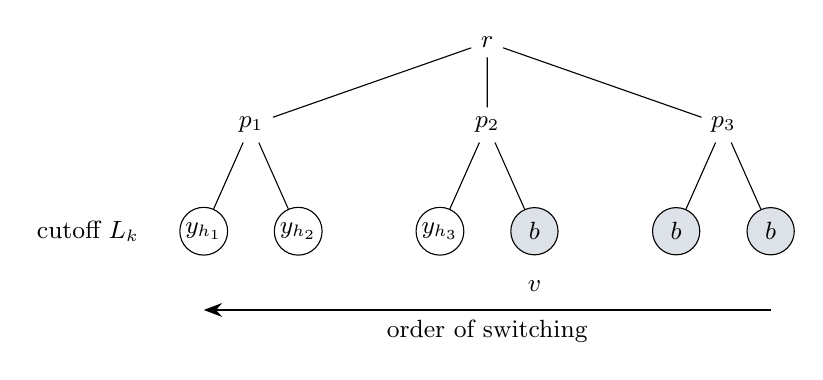
\begin{tikzpicture}[>=Stealth,
  point/.style={circle,draw,minimum size=6mm,inner sep=1pt},
  untouched/.style={point,fill=white},
  switched/.style={point,fill=linkblue!15},
  every node/.style={font=\small}]
\node (root) at (0,2.4) {$r$};
\node (p1) at (-3,1.35) {$p_1$};
\node (p2) at (0,1.35) {$p_2$};
\node (p3) at (3,1.35) {$p_3$};
\draw (root)--(p1) (root)--(p2) (root)--(p3);
\node[untouched] (h1) at (-3.6,0) {$y_{h_1}$};
\node[untouched] (h2) at (-2.4,0) {$y_{h_2}$};
\node[untouched] (h3) at (-.6,0) {$y_{h_3}$};
\node[switched] (v) at (.6,0) {$b$};
\node[switched] (h5) at (2.4,0) {$b$};
\node[switched] (h6) at (3.6,0) {$b$};
\draw (p1)--(h1) (p1)--(h2) (p2)--(h3) (p2)--(v) (p3)--(h5) (p3)--(h6);
\node[below=2mm of v] {$v$};
\node[anchor=east] at (-4.3,0) {cutoff $L_k$};
\draw[->,thick] (3.6,-1.0)--(-3.6,-1.0)
 node[midway,below] {order of switching};
\end{tikzpicture}

\caption{An ideal cutoff state immediately after the block below $v$
has switched. Earlier nodes retain their labels; $v$ and the nodes to
its right have output $b$. Each parent applies its map to the weighted
average of its children. The diagram displays a two-level example of
this rule; in a deeper tree the same evaluation continues up to the root.
The coefficients on the earlier labels specify $\theta^v$, and their
residual mass multiplies $b$.}
\label{fig:cutoff}
\end{figure}

\section{Switching leaves and completing the proof}
\label{sec:switching}

Fix the tree supplied by Proposition~\ref{prop:tree-data}.
Write $v\preceq s$ when $v=s$ or $v\prec s$.
For $N\geq 1$, set
\[
  \mathcal T_N=\bigcup_{k=0}^{N}L_k,
  \qquad
  B_N(v)=\{s\in L_N:v\preceq s\}
  \quad(v\in\mathcal T_N).
\]
The set $B_N(v)$ is a consecutive block in the ordering of $L_N$, and
\[
  \sum_{s\in B_N(v)}W_s=W_v.
\]
We first show that some path in each finite truncation has all its
functionals large on one vector.

\begin{proposition}[A finite witness]
\label{prop:finite-witness}
For every $N\geq 1$, there are a leaf $s\in L_N$ and a vector $d\in B_Y$
such that
\[
  f_v(d)\geq \frac12
  \qquad
  (r\ne v\preceq s).
\]
\end{proposition}

\begin{proof}
Fix $N$. All the maps, weights, functionals, and budgets in $\mathcal T_N$
are already fixed. Put
\[
  M_k=\min\{e_v:v\in L_1\cup\cdots\cup L_k\}
  \qquad(1\leq k\leq N).
\]

\emph{Choosing a common terminal point.}
For each $v\in\mathcal T_N\setminus\{r\}$, use the parameter
$\theta^v\in\Theta_v$ from Section~\ref{sec:tree}: it assigns the actual
weight $\alpha_h$ to each earlier retained candidate $h\in I_v$, and zero
to each earlier discarded candidate. The point
\[
  q_v=Z_v(\theta^v)
      =\operatorname*{w-lim}_{j\to\mathcal U}Q_v(b_j;\theta^v)
\]
belongs to $E_v$ by \eqref{eq:tree-detector-set}. By \eqref{eq:tree-conditions},
$f_v(y_v-q_v)\geq 1-e_v$. The definition of this weak ultrafilter limit
therefore gives
\[
  \bigl\{j\in\N:
       f_v\bigl(y_v-Q_v(b_j;\theta^v)\bigr)\geq 1-2e_v\bigr\}
       \in\mathcal U.
\]
There are only finitely many such conditions. Moreover,
\eqref{eq:map-displacement} and the approximate fixed point property of
$(b_j)$ give
\[
  \sum_{u\in\mathcal T_N}\norm{G_u(b_j)-b_j}\longrightarrow 0.
\]
Intersecting the finitely many ultrafilter members above with a suitable
cofinite set, choose one $j$ and write $b=b_j$ so that
\begin{align}
  f_v\bigl(y_v-Q_v(b;\theta^v)\bigr)
     &\geq 1-2e_v
     &&(v\in\mathcal T_N\setminus\{r\}),
     \label{eq:terminal-detection}\\
  D_N:=\sum_{u\in\mathcal T_N}\norm{G_u(b)-b}
     &\leq M_N.
     \label{eq:truncation-displacement}
\end{align}

\emph{The switching experiment.}
Initially assign the output $H_s=y_s$ to each leaf $s\in L_N$.
Switch these outputs one at a time to $H_s=b$, proceeding from right to
left. At each stage calculate every other output by
\eqref{eq:tree-rule}. All outputs belong to $K$.
For $v\in\mathcal T_N\setminus\{r\}$, let $U_v$ and $V_v$ be the root
outputs immediately before and immediately after the whole block
$B_N(v)$ is switched.

We need two estimates for subtrees whose leaves are all in the same
state. If none of the leaves below $h\in L_k$ have switched, then
\begin{equation}
  \norm{H_h-y_h}
     \leq \varepsilon_{k,N}:=\sum_{d=k}^{N-1}\tau_d.
  \label{eq:untouched-error}
\end{equation}
Here and below an empty sum is zero. At a leaf this is an equality.
For an internal node, nonexpansiveness and \eqref{eq:child-average}
give the induction step
\begin{align*}
  \norm{H_h-y_h}
  &\leq
    \norm*{\sum_{\widehat u=h}\alpha_u H_u-x}\\
  &\leq
    \sum_{\widehat u=h}\alpha_u\norm{H_u-y_u}
       +\norm*{\sum_{\widehat u=h}\alpha_u y_u-x}
   \leq \varepsilon_{k+1,N}+\tau_k.
\end{align*}
The tolerance schedule \eqref{eq:tree-tolerance} yields, for $k\geq 1$
and every $v\in L_k$,
\begin{equation}
  \varepsilon_{k,N}
    \leq M_k\sum_{d=k}^{\infty}2^{-d-1}
    =2^{-k}M_k
    \leq e_v.
  \label{eq:uniform-level-error}
\end{equation}
Thus the error in \eqref{eq:untouched-error} is at most $e_v$ for every
unchanged node at depth $k$, regardless of which $v\in L_k$ is used in
the comparison.

If all the leaves below $h$ have switched, put
$\delta_u=\norm{G_u(b)-b}$. At each internal node of that subtree,
\[
  \norm{H_u-b}
    \leq \sum_{\widehat w=u}\alpha_w\norm{H_w-b}+\delta_u.
\]
The error at each leaf is zero. Iteration gives
\begin{equation}
  \norm{H_h-b}
    \leq
      \sum_{\substack{u\in\mathcal T_N\setminus L_N\\h\preceq u}}
           \frac{W_u}{W_h}\delta_u
    \leq D_N
    \leq M_N.
  \label{eq:transmitted-error}
\end{equation}
The coefficients $W_u/W_h$ are products of weights below $h$ and are
at most one.

\emph{Detection of an entire block.}
Fix $v\in L_k$, where $1\leq k\leq N$, and consider the stage immediately
before its block switches. Its output is within $e_v$ of $y_v$ by
\eqref{eq:untouched-error}--\eqref{eq:uniform-level-error}.
Let $p_0=r,p_1,\ldots,p_k=v$ be the path to $v$, and put
$A_i=\norm{H_{p_i}-y_v}$ at this stage. Since every off-path child output
and $y_v$ lie in the diameter-one set $K$, nonexpansiveness gives
\[
  A_i\leq
     \alpha_{p_{i+1}}A_{i+1}
       +(1-\alpha_{p_{i+1}})
       +\norm{G_{p_i}(y_v)-y_v}
       \qquad(0\leq i<k).
\]
The off-path contributions telescope:
\[
 \sum_{i=0}^{k-1}W_{p_i}(1-\alpha_{p_{i+1}})
 =\sum_{i=0}^{k-1}(W_{p_i}-W_{p_{i+1}})=1-W_v.
\]
Unwinding the recurrence and using \eqref{eq:tree-conditions}, we obtain
\begin{align}
  \norm{U_v-y_v}
   &\leq
      W_v e_v+(1-W_v)
       +\sum_{i=0}^{k-1}W_{p_i}\norm{G_{p_i}(y_v)-y_v}
       \notag\\
   &\leq 1-W_v+2e_v.
   \label{eq:before-block}
\end{align}

Immediately after the block has switched, precisely the level-$k$
nodes strictly to the left of $v$ have unchanged leaf blocks. By
\eqref{eq:uniform-level-error}, their outputs are within $e_v$ of their
labels $y_h$. The outputs at all the other level-$k$ nodes are within
$M_N\leq e_v$ of $b$ by \eqref{eq:transmitted-error}.
The ideal level-$k$ assignment consisting of these $y_h$ on the left
and $b$ elsewhere has root output $Q_v(b;\theta^v)$ by
\eqref{eq:prediction-cutoff}. The sensitivity estimate
\eqref{eq:tree-sensitivity} and $\sum_{h\in L_k}W_h=1$ therefore imply
\begin{equation}
  \norm{V_v-Q_v(b;\theta^v)}\leq e_v.
  \label{eq:after-block}
\end{equation}
Together, \eqref{eq:terminal-detection}, \eqref{eq:before-block}, and
\eqref{eq:after-block} give
\begin{align}
  f_v(U_v-V_v)
   &\geq f_v\bigl(y_v-Q_v(b;\theta^v)\bigr)
               -\norm{U_v-y_v}-\norm{V_v-Q_v(b;\theta^v)}
               \notag\\
   &\geq (1-2e_v)-(1-W_v+2e_v)-e_v
    =W_v-5e_v.
  \label{eq:block-detection}
\end{align}

\emph{A common witness along one path.}
For a single leaf $s$, only its output changes during its switch.
By \eqref{eq:tree-sensitivity},
\[
  \norm{U_s-V_s}\leq W_s\norm{y_s-b}\leq W_s.
\]
Since $W_s>0$ and both root outputs belong to $K$, the vector
\[
  d_s=\frac{U_s-V_s}{W_s}
\]
belongs to $B_Y$. The successive root differences over a consecutive
block telescope, so
\[
  \sum_{s\in B_N(v)}W_s d_s=U_v-V_v.
\]
Applying $f_v$ to this identity and using \eqref{eq:block-detection}
yields
\begin{equation}
  \sum_{s\in B_N(v)}W_s\bigl(1-f_v(d_s)\bigr)
     =W_v-f_v(U_v-V_v)
     \leq 5e_v.
  \label{eq:weighted-deficit}
\end{equation}
Each summand is nonnegative, because $\norm{f_v}\leq 1$ and
$\norm{d_s}\leq 1$. Summing over the non-root nodes and interchanging the
two finite sums gives
\begin{equation}
  \sum_{s\in L_N}W_s
       \sum_{r\ne v\preceq s}\bigl(1-f_v(d_s)\bigr)
    \leq 5\sum_{v\in\mathcal T_N\setminus\{r\}}e_v
    \leq \frac{5}{128}.
  \label{eq:total-deficit}
\end{equation}
If a leaf $s$ has $f_v(d_s)\leq 1/2$ for any non-root node $v$ on its
path, its inner sum in \eqref{eq:total-deficit} is at least $1/2$. Consequently,
the total weight of all such leaves is at most $5/64$. Since the leaf
weights sum to one, some leaf has $f_v(d_s)>1/2$ for every non-root
node $v$ on its path. This proves the proposition.
\end{proof}

\begin{proof}[Proof of Theorem~\ref{thm:main}]
Suppose a counterexample exists. The reduction and constructions in
Sections~\ref{sec:prelim}--\ref{sec:tree} give the fixed infinite tree to
which Proposition~\ref{prop:finite-witness} applies.
Call a node $v$ \emph{feasible} if some $d\in B_Y$ satisfies
\[
  f_u(d)\geq\frac12\qquad(r\ne u\preceq v).
\]
The root is feasible, and every ancestor of a feasible node is feasible.
Proposition~\ref{prop:finite-witness} gives a feasible node at every depth.
These nodes therefore form a finitely branching tree with arbitrarily
great depth. Starting from the root, choose a child having feasible
descendants at arbitrarily great depths, and repeat. Such a child always
exists because each node has finitely many children. This produces a
branch $r,v_1,v_2,\ldots$, with $v_k\in L_k$, all of whose nodes are
feasible.

For each $k\geq 1$, the set
\[
  C_k=\{d\in B_Y:f_{v_i}(d)\geq 1/2\text{ for }1\leq i\leq k\}
\]
is nonempty and weakly closed in $B_Y$, and $C_{k+1}\subseteq C_k$.
The normalized differences used in Proposition~\ref{prop:finite-witness}
are controlled in the whole unit ball $B_Y$. Reflexivity supplies weak
compactness of this ball, as established in Section~\ref{sec:prelim}.
It follows that there is one vector
\begin{equation}
  d\in\bigcap_{k=1}^{\infty}C_k,
  \qquad
  f_{v_k}(d)\geq\frac12\quad(k\geq 1).
  \label{eq:common-branch-vector}
\end{equation}

On the other hand, the functionals on every branch converge pointwise
to zero on $Y$. Indeed, for fixed $i,j$ and $k\geq\max\{i,j\}$,
\eqref{eq:tree-conditions} and $\diam K=1$ give
\[
  1-e_{v_k}\leq f_{v_k}(y_{v_k}-z_i)\leq 1,
  \qquad
  1-e_{v_k}\leq f_{v_k}(y_{v_k}-z_j)\leq 1.
\]
Subtracting these inequalities yields
\[
  \abs{f_{v_k}(z_i-z_j)}\leq e_{v_k}\longrightarrow 0,
\]
where the convergence follows from the summability of the budgets.
The linear span of the differences $z_i-z_j$ is dense in
$Y=\overline{\operatorname{span}}(K-K)$. Hence the bound
$\norm{f_{v_k}}\leq 1$ extends this convergence to every $d'\in Y$:
for any vector $a$ in that span,
\[
  \abs{f_{v_k}(d')}\leq\norm{d'-a}+\abs{f_{v_k}(a)},
\]
and one first lets $k$ tend to infinity and then lets $a$ approach $d'$.
In particular $f_{v_k}(d)\to 0$, contradicting
\eqref{eq:common-branch-vector}. The assumed counterexample cannot exist.
\end{proof}

\appendix
\section{Separation and compactness}\label{app:foundations}

Here $X$ is a general real normed space, as in Lemma~\ref{lem:weak-facts}.

\begin{proof}[Proof of Lemma~\ref{lem:weak-facts}]
We begin with the Hahn--Banach extension argument underlying the first two assertions.
Suppose that a linear functional $\ell$ on a subspace $M$ is dominated by a
continuous sublinear function $p$ on $X$. To extend it to $M+\R b$, where
$b\notin M$, choose its value at $b$ in the interval
\[
 \sup_{a\in M}\bigl(\ell(a)-p(a-b)\bigr)
 \ \leq\ \ell(b)\ \leq\
 \inf_{c\in M}\bigl(p(c+b)-\ell(c)\bigr).
\]
This interval is nonempty because
$\ell(a)+\ell(c)\leq p(a+c)\leq p(a-b)+p(c+b)$.
Its endpoints are finite, as is seen by setting $a=0$ or $c=0$ in this
inequality. The displayed bounds give domination on $a+b$ and $a-b$;
positive homogeneity then gives domination on $a+tb$ for every real $t$.
Unions of chains of dominated extensions remain dominated extensions, so
Zorn's Lemma gives an extension to $X$. It is continuous because domination
of both $v$ and $-v$ bounds its absolute value near zero.
Applying this construction with $p=\norm{\cdot}$ and
$\ell(tv)=t\norm{v}$ gives a norming functional (use the zero functional
when $v=0$). In particular,
\[
             \norm{v}=\sup_{f\in X^*,\ \norm{f}\leq1}f(v).
\]

For separation, let $q$ lie outside a nonempty norm-closed convex set $D$.
Choose $\rho>0$ such that the open convex set
$U=D+\{v:\norm{v}<\rho\}$ still excludes $q$, and fix $u\in U$.
The gauge
\[
 p(v)=\inf\{t>0:v\in t(U-u)\}
\]
is finite, nonnegative, positively homogeneous, and subadditive.
For the last property, if $v\in s(U-u)$ and $w\in t(U-u)$, convexity gives
$v+w\in(s+t)(U-u)$, and one takes infima.
Since $U-u$ is open, convex, and contains zero, $\{v:p(v)<1\}=U-u$:
one inclusion follows from convexity, and the other by extending a little
past a given point along its ray using openness.
A ball about zero contained in $U-u$ gives $p(v)\leq c\norm{v}$ for some
$c$; subadditivity then makes $p$ continuous.
On the line through $q-u$, the functional taking the value $p(q-u)$ at
$q-u$ is dominated by $p$; for negative multiples this follows from
$-p(q-u)\leq p(u-q)$. Its extension $f$ therefore satisfies
\[
             f(z-u)<1\leq f(q-u)\qquad(z\in U).
\]
In particular $f\ne0$, and taking the supremum over the ball of radius
$\rho$ added to any $d\in D$ gives
$f(d)+\rho\norm{f}\leq f(q)$. Thus $f$ separates $q$ from $D$ with a
positive gap. This proves weak closedness of $D$. Applied to closed balls
it proves weak lower semicontinuity of the norm. Separation also shows
that the weak closure of a convex set equals its norm closure.
On $X^r$, equipped with the maximum norm, every continuous linear
functional has the form $\sum_{i=1}^r f_i(x_i)$, with $f_i\in X^*$,
by restriction to the coordinate subspaces. This proves the assertion
about the finite-product topology and allows the same separation argument
there.

Here are the compactness details. A proper filter is a family of subsets
closed under finite intersections and supersets, containing the whole
space but not the empty set. By Zorn's Lemma it extends to a maximal proper
filter, called an ultrafilter. For every subset an ultrafilter contains
either that subset or its complement: if the subset cannot be added while
preserving the filter property, an existing filter member misses it.
An ultrafilter converges to a point when it contains every neighborhood
of that point. In a compact space it converges: the closures of its members
have the finite intersection property, and any point in their intersection
is a limit by the preceding either-or property. Limits are unique in a
Hausdorff space. Conversely, if every ultrafilter converges, extend any
family of closed sets with the finite intersection property to an
ultrafilter; its limit belongs to all those sets. This is the closed-set
criterion for compactness. An ultrafilter on a product of compact spaces
has a limit in each coordinate, and the tuple of these limits is its
limit, since a basic product neighborhood restricts only finitely many
coordinates. This proves product compactness.

Now let $D\subseteq X$ be bounded, norm closed, and convex, with $X$
reflexive. Given an ultrafilter $\mathcal V$ on $D$, each bounded real
evaluation has a limit in a compact interval, and
\[
             L(f)=\lim_{\mathcal V} f(d)\qquad(f\in X^*)
\]
defines a linear functional with $\abs{L(f)}\leq M\norm{f}$, where
$M=\sup_{d\in D}\norm{d}$. Linearity follows by intersecting the filter
members on which each of two evaluations is close to its limit.
Reflexivity supplies $a\in X$ with $L(f)=f(a)$ for every $f$.
Thus $\mathcal V$ converges weakly to $a$, and weak closedness gives
$a\in D$. The ultrafilter criterion proves weak compactness.
\end{proof}

\bibliographystyle{plainnat}
\bibliography{references}
\end{document}
